\chapter{Applikation Mockups}
Dette kapitel beskriver de mockups, der er blevet udarbejdet i samarbejde med Rambøll, for at have et fælles udgangspunkt for user interfacet og flowet gennem applikationen. \\

\section{Login}\label{sec:LoginMock}
På figur \ref{fig:LoginMock} ses login siden for appliaktionen. Her skal brugeren indtaste brugernavn og password for at få adgang til Rambøll Tilyns App.
\begin{figure}[H]
	\centering
	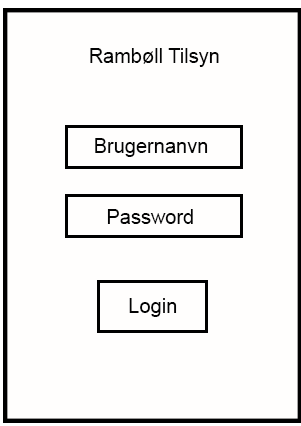
\includegraphics[width=0.4\linewidth]{MockUps/Mock/Ramboell-Login}
	\caption{Login siden for Rambøll Tilsyns App}
	\label{fig:LoginMock}
\end{figure}

\clearpage

\section{Startside}\label{sec:StartMock}
På figur \ref{fig:StartMock} ses startsiden for Rambøll Tilsyns App. Her kan brugeren vælge, hvilket projekt der ønskes at arbejdes på eller bruger kan vælge at åbne submenuen i øverste højre hjørne.
\begin{figure}[H]
	\centering
	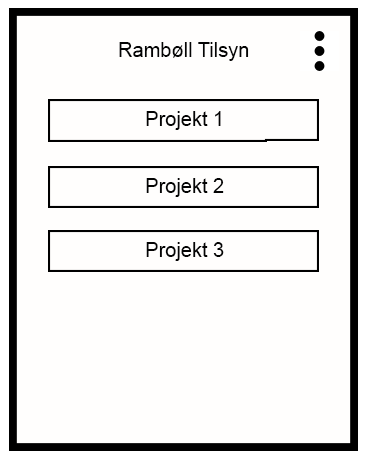
\includegraphics[width=0.4\linewidth]{MockUps/Mock/Ramboell-Startside}
	\caption{Startsiden for Rambøll Tilsyns App}
	\label{fig:StartMock}
\end{figure}

\section{Startside submenu}\label{sec:StartSubMock}
På figur \ref{fig:StartSubMock} ses startsidens submenu for Rambøll Tilsyns App. Her kan brugeren vælge at oprette et nyt projekt, oprette ny bruger eller redigere sin egen bruger.

\begin{figure}[H]
	\centering
	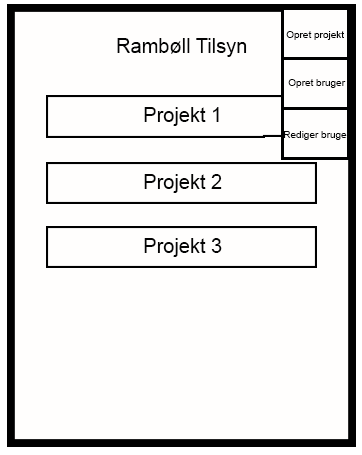
\includegraphics[width=0.4\linewidth]{MockUps/Mock/Ramboell-Startside-Sub}
	\caption{Startsiden med åben submenu for Rambøll Tilsyns App}
	\label{fig:StartSubMock}
\end{figure}

\clearpage

\section{Opret projekt}\label{sec:OpretProjektMock}
På figur \ref{fig:OpretProjektMock} ses opret projekt siden, hvor brugeren kan oprette nye projekter.

\begin{figure}[H]
	\centering
	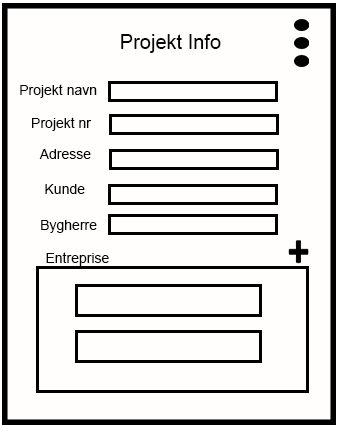
\includegraphics[width=0.4\linewidth]{MockUps/Mock/Ramboell-ProjektInfo}
	\caption{Opret projekt siden for Rambøll Tilsyns App}
	\label{fig:OpretProjektMock}
\end{figure}

\section{Opret bruger}\label{sec:OpretBrugerMock}
På figur \ref{fig:OpretBrugerMock} ses opret bruger siden, hvor brugeren kan oprette nye brugere til systemet.

\begin{figure}[H]
	\centering
	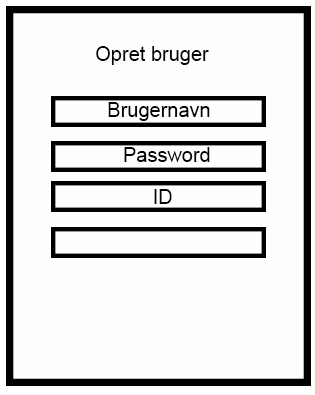
\includegraphics[width=0.4\linewidth]{MockUps/Mock/Ramboell-OpretBruger}
	\caption{Opret bruger siden for Rambøll Tilsyns App}
	\label{fig:OpretBrugerMock}
\end{figure}

\clearpage

\section{Rediger bruger}\label{sec:RedigerBrugerMock}
På figur \ref{fig:RedigerBrugerMock} ses rediger bruger siden, hvor brugeren kan redigere sin egen bruger.

\begin{figure}[H]
	\centering
	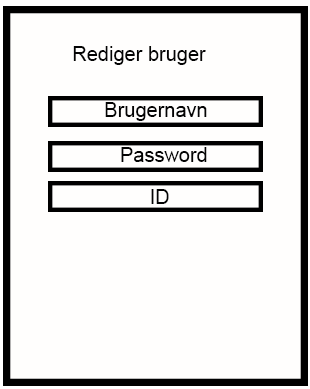
\includegraphics[width=0.4\linewidth]{MockUps/Mock/Ramboell-RedigerBruger}
	\caption{Rediger bruger siden for Rambøll Tilsyns App}
	\label{fig:RedigerBrugerMock}
\end{figure}

\section{Projektside}\label{sec:ProjektsideMock}
På figur \ref{fig:ProjektsideMock} ses projektsiden, hvor brugeren vælger hvilken type registrering, der skal laves eller om bruger ønsker at se tilsynsrapporterne for projektet.

\begin{figure}[H]
	\centering
	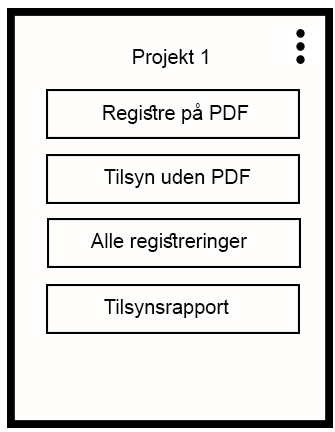
\includegraphics[width=0.4\linewidth]{MockUps/Mock/Ramboell-Registrer}
	\caption{Projektsiden for Rambøll Tilsyns App}
	\label{fig:ProjektsideMock}
\end{figure}

\clearpage

\section{Projektside med flere entrepriser}\label{sec:ProjektsideEntrepriseMock}
På figur \ref{fig:ProjektsideEntrepriseMock} ses projektsiden, hvis der er mere end én entreprise. Her har brugeren mulighed for vælge, hvilken entreprise der ønskes at registreres på.

\begin{figure}[H]
	\centering
	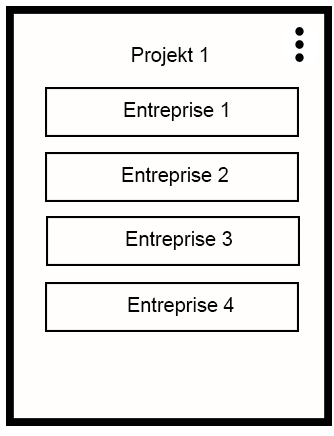
\includegraphics[width=0.4\linewidth]{MockUps/Mock/Ramboell-Entreprise}
	\caption{Projektsiden med submenu for Rambøll Tilsyns App}
	\label{fig:ProjektsideEntrepriseMock}
\end{figure}

\section{Projektside submenu}\label{sec:ProjektsideSubMock}
På figur \ref{fig:ProjektsideSubMock} ses projektsiden med submenuen åben. Her har brugeren mulighed for at redigere projektinfo for det valgte projekt.

\begin{figure}[H]
	\centering
	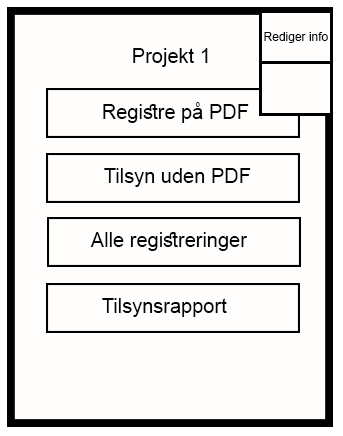
\includegraphics[width=0.4\linewidth]{MockUps/Mock/Ramboell-Registrer-sub}
	\caption{Projektsiden med submenu for Rambøll Tilsyns App}
	\label{fig:ProjektsideSubMock}
\end{figure}

\section{Projektinfo}\label{sec:ProjektinfoMock}
På figur \ref{fig:ProjektinfoMock} ses projektinfo siden. Her har brugeren mulighed for at se alt information for det valgte projekt.

\begin{figure}[H]
	\centering
	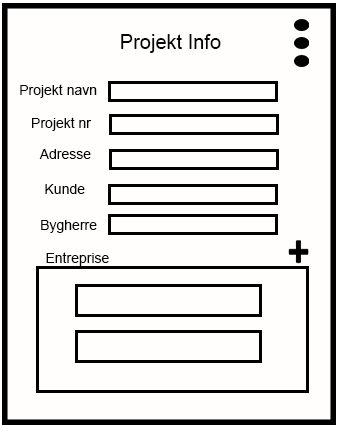
\includegraphics[width=0.4\linewidth]{MockUps/Mock/Ramboell-ProjektInfo}
	\caption{Projektinfo for Rambøll Tilsyns App}
	\label{fig:ProjektinfoMock}
\end{figure}

\section{Projektinfo submenu}\label{sec:ProjektinfoSubMock}
På figur \ref{fig:ProjektinfoSubMock} ses projektinfo siden med submenuen åben. Her har brugeren mulighed for at redigere projektinfo for det valgte projekt

\begin{figure}[H]
	\centering
	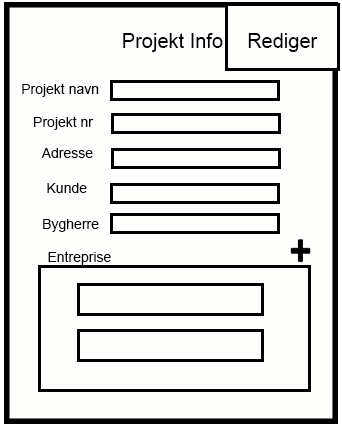
\includegraphics[width=0.4\linewidth]{MockUps/Mock/Ramboell-ProjektInfo-Sub}
	\caption{Projektinfo siden med submenu for Rambøll Tilsyns App}
	\label{fig:ProjektinfoSubMock}
\end{figure}

\clearpage

\section{Registrering på PDF}\label{sec:RegPaaPDFMock}
På figur \ref{fig:RegPaaPDFMock} ses registrering på PDF siden. Her har brugeren mulighed for at lave registreringer på en PDF tegning til det valgte projekt.

\begin{figure}[H]
	\centering
	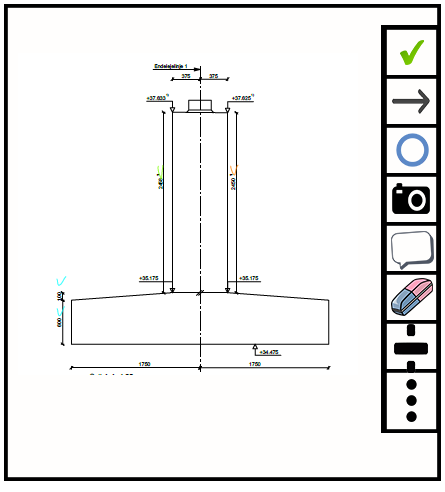
\includegraphics[width=0.4\linewidth]{MockUps/Mock/Ramboell-PDF-Reg}
	\caption{Registre på PDF siden for Rambøll Tilsyns App}
	\label{fig:RegPaaPDFMock}
\end{figure}


\section{Registrering på PDF submenu}\label{sec:RegPaaPDFSubMock}
På figur \ref{fig:RegPaaPDFSubMock} ses registrering på PDF siden med submenuen åben. Her har brugeren mulighed for at afslutte registreringen.

\begin{figure}[H]
	\centering
	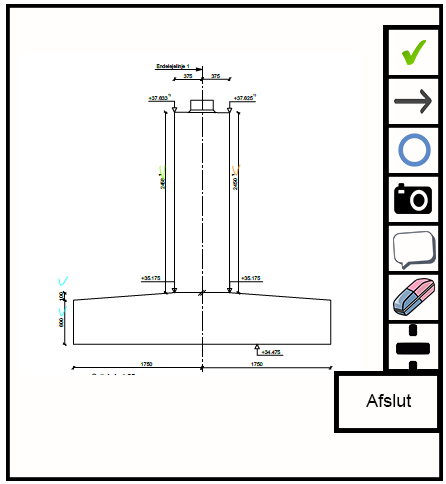
\includegraphics[width=0.4\linewidth]{MockUps/Mock/Ramboell-PDF-Reg-sub}
	\caption{Registre på PDF siden med submenu for Rambøll Tilsyns App}
	\label{fig:RegPaaPDFSubMock}
\end{figure}

\clearpage

\section{Registrering uden PDF}\label{sec:RegUdenPDFMock}
På figur \ref{fig:RegUdenPDFMock} ses registrering uden PDF siden. Her har brugeren mulighed for at lave registreringer uden en PDF tegning til det valgte projekt.

\begin{figure}[H]
	\centering
	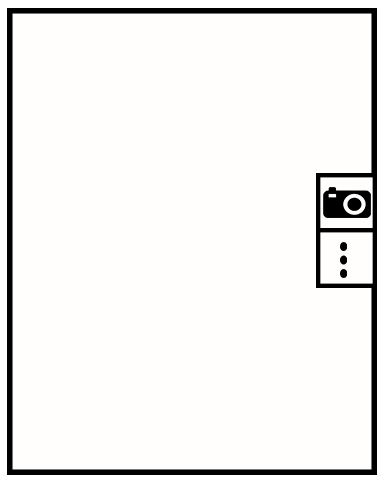
\includegraphics[width=0.4\linewidth]{MockUps/Mock/Ramboell-TilsynUden}
	\caption{Registre uden PDF siden for Rambøll Tilsyns App}
	\label{fig:RegUdenPDFMock}
\end{figure}


\section{Registrering uden PDF submenu}\label{sec:RegUdenPDFSubMock}
På figur \ref{fig:RegUdenPDFSubMock} ses registrering uden PDF siden med submenuen åben. Her har brugeren mulighed for at afslutte registreringen.

\begin{figure}[H]
	\centering
	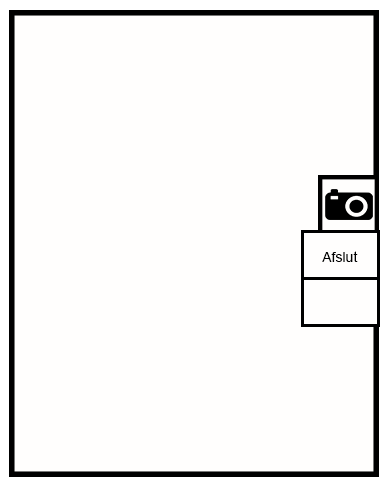
\includegraphics[width=0.4\linewidth]{MockUps/Mock/Ramboell-TilsynUden-sub}
	\caption{Registre uden PDF siden med submenu for Rambøll Tilsyns App}
	\label{fig:RegUdenPDFSubMock}
\end{figure}

\clearpage

\section{Rediger billede objekt}\label{sec:RedigerBilledeMock}
På figur \ref{fig:RedigerBilledeMock} ses rediger billede vinduet. Her har brugeren mulighed for at se det billede og teksten tilhørende billede objektet.

\begin{figure}[H]
	\centering
	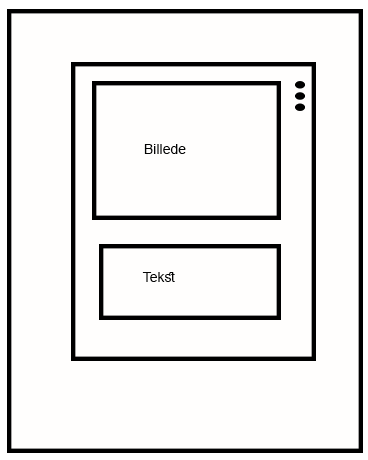
\includegraphics[width=0.4\linewidth]{MockUps/Mock/Ramboell-RedigerBilledeOpbjekt}
	\caption{Redigerer billede objekt vinduet for Rambøll Tilsyns App}
	\label{fig:RedigerBilledeMock}
\end{figure}

\section{Rediger billede objekt submenu}\label{sec:RedigerBilledeSubMock}
På figur \ref{fig:RedigerBilledeSubMock} ses rediger vinduet siden med submenuen åben. Her har brugeren mulighed for at redigere det billede, der er blevet taget eller redigerer billedeteksten.

\begin{figure}[H]
	\centering
	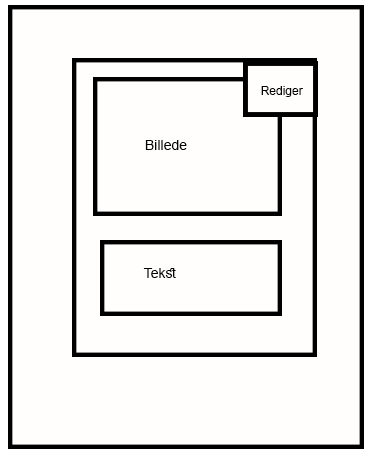
\includegraphics[width=0.4\linewidth]{MockUps/Mock/Ramboell-RedigerBilledeOpbjekt-Sub}
	\caption{Redigere billede objekt vinduet med submenu for Rambøll Tilsyns App}
	\label{fig:RedigerBilledeSubMock}
\end{figure}

\clearpage

\section{Preview}\label{sec:PreviewMock}
På figur \ref{fig:PreviewMock} ses preview siden. Her har brugeren mulighed for at se et preview af tilsynsrapporten lavet ved registrering uden PDF.

\begin{figure}[H]
	\centering
	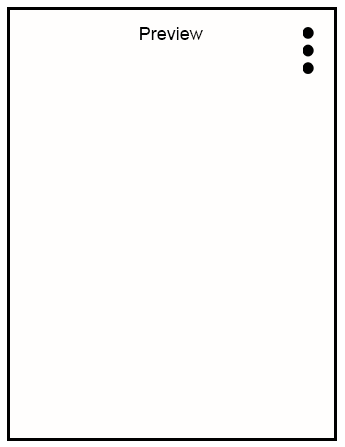
\includegraphics[width=0.4\linewidth]{MockUps/Mock/Ramboell-Preview}
	\caption{Preview siden for Rambøll Tilsyns App}
	\label{fig:PreviewMock}
\end{figure}

\section{Preview submenu}\label{sec:PreviewSubMock}
På figur \ref{fig:PreviewSubMock} ses preview siden med submenuen åben. Her har brugeren mulighed for at eksporterer tilsynsrapporten.

\begin{figure}[H]
	\centering
	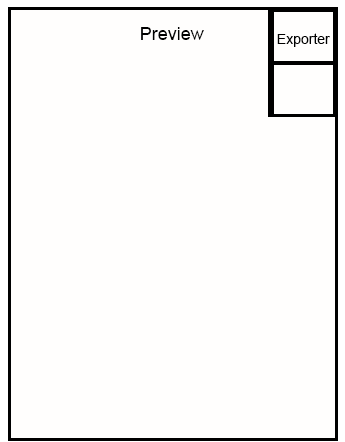
\includegraphics[width=0.4\linewidth]{MockUps/Mock/Ramboell-Preview-Sub}
	\caption{Preview siden med submenu for Rambøll Tilsyns App}
	\label{fig:PreviewSubMock}
\end{figure}
